\chapter{Wprowadzenie do fingerprintingu}

\section{Podstawowe pojęcia}

\subsection{Nomenklatura używana w tej pracy}
Pisząc o odcisku palca użyto (także w tytule pracy) ogólnie przyjętego skrótu
myślowego, oznaczającego odbitkę linii papilarnych, czyli formę językową
uznawaną za poprawną przez specjalistów od daktyloskopii.

Użycie formy językowej ,,odcisk palca'' w terminie ,,cyfrowy odcisk palca'' ma
wiele sensu. Jeszcze bez zdefiniowania tego specjalistycznego terminu, możemy
domyślić się, co oznacza. Oczywiście wynika to z faktu, że cyfrowy odcisk palca
i analogowy odcisk palca są ze sobą w pewien sposób powiązane (koncepcja
cyfrowego odcisku palca czerpie z wartości wynikających ze stosowania odbitek
ludzkich linii papilarnych w dziedzinie kryminalistyki).

Angielskie słowo ,,fingerprint'' tłumaczy się jako odcisk palca, jednakże w
zagranicznych publikacjach dotyczących cyfrowego odcisku palca rzadko występuje
termin ,,digital fingerprint''. Kontekst użycia jest na tyle wyraźny, że użycie
samego ,,fingerprint'' jest wystarczające.

Zachodnie nazewnictwo ma tę przewagę, że jest zdecydowanie bardziej kompaktowe.
Także w przypadku słowotwórczego zabiegu \emph{fingerprinting}, oznaczającego
czynność; szukając polskiego odpowiednika musielibyśmy sięgnąć po ,,cyfrowe
znakowanie''. Z uwagi na tę kompaktowość i łatwość użycia, w pracy preferowane
będzie użycie oryginalnej nomenklatury.

\subsection{Definicje}
W kolejnych punktach zawarto najważniejsze definicje i powiązane pojęcia, które
będą używane w przeciągu całej pracy.

\subsubsection{Fingerprint}
Wektor cech pozwalający zidentyfikować dowolny zbiór danych.

Aby fingerprint pełnił praktyczną funkcję identyfikacyjną, tak jak odbitka
ludzkich linii papilarnych pełni praktyczną funkcję identyfikacyjną, często
stosuje się algorytm, który kojarzy wektor cech z określonej długości (zwykle
krótkim) ciągiem bajtów (identyfikatorem; można go także rozumieć jako
etykieta). Takim algorytmem może być na przykład wysokiej wydajności funkcja
skrótu (niekoniecznie zdatna do zastosowań kryptograficznych---na przykład
MurmurHash). W niektórych źródłach można także spotkać się z taką definicją, że
fingerprint to już sam wynik wyżej wspomnianego algorytmu. Taka definicja nie
zmienia istoty fingerprintu, ale jest zdecydowanie mniej przydatna w kontekście
fingerprintingu urządzeń podłączonych do Internetu i przeglądarek internetowych,
czego dotyczy niniejsza praca.

\subsubsection{Fingerprint urządzenia podłączonego do Internetu}
Wektor cech pozwalający zidentyfikować urządzenie podłączone do Internetu.

\subsubsection{Instalacja przeglądarki internetowej}
Instalacja na konkretnym urządzeniu. W przypadku zmiany ustawień, konfiguracji i
liczby pluginów oraz aktualizacji przeglądarki, instalacja przeglądarki
pozostaje ciągle tą samą instalacją.

\subsubsection{Fingerprint przeglądarki internetowej}
Wektor cech pozwalający zidentyfikować instalację przeglądarki internetowej.

\subsection{Właściwości fingerprintu}
Ludzkie linie papilarne są na ogół niepowtarzalne, niezmienne i nieusuwalne. Z
wartości wynikających ze stosowania ich odbitek w swojej dziedzinie badawczej
czerpie (także etymologicznie) koncepcja fingerprintu i dlatego też fingerprint
z dobrze dobranymi cechami będzie odzwierciedlać podobne właściwości.

W przypadku fingerprintingu urządzeń podłączonych do Internetu i przeglądarek
internetowych najważniejszymi ich właściwościami są unikalność / różnorodność
(niepowtarzalność) oraz stabilność (niezmienność), przy czym zwiększenie
unikalności lub stabilności ma najczęściej negatywny wpływ na drugi parametr.

Jedną ze stosowanych\footnote{Metrykę tę stosowało na przykład badanie ,,How
	Unique Is Your Web Browser?'' Electronic Frontier Foundation; w momencie
pisania pracy jedno z największych badań tego typu.} metod pomiaru unikalności
fingerprintu urządzeń i przeglądarek jest entropia Shannona.

\subsubsection{Entropia Shannona}
Wartość entropii można rozumieć jako liczbę pytań binarnych potrzebnych do
sklasyfikowania losowo wybranego elementu z danego zbioru. Zatem entropia
Shannona zbioru \(D\) z etykietami \(\{l_{0}, l_{1}, \dots, l_{n - 1}\}\) wyraża
się wzorem \[H(D) = -{\sum_{i = 0}^{n - 1}{p(l_{i})\log_{2}{p(l_{i})}}}\] gdzie
\(p(l_{i})\) to wyrażona ułamkiem częstość \(x \in D\) mającego etykietę
\(l_{i}\). W przypadku w którym każda etykieta występuje tak samo często
entropia ma wartość maksymalną równą \(\log_{2}{n}\).

\paragraph{Przykład}
Jeśli zbiór fingerprintów przeglądarek internetowych ma \(32\) bity entropii, to
w przypadku losowego wyboru jednego z nich oczekujemy, że w najlepszym przypadku
tylko \(1\) na \(4294967295\) przeglądarek będzie miała taki sam fingerprint.

\subsubsection{Stabilność}
W przypadku dodania kolejnej cechy do wektora cech, identyfikującego urządzenie
lub przeglądarkę, zwykle zwiększy to entropię, ale także zmniejszy stabilność
fingerprintu. Dzieje się tak ponieważ jest to kolejna rzecz, która może zmienić
się w czasie. Jeśli jedną z cech wejściowych jest wersja oprogramowania
urządzenia lub wersja przeglądarki (która zwykle zmienia się parę razy w ciągu
roku), to kolejne fingerprinty mogą odbiegać od siebie i naiwny klasyfikator,
korzystający z algorytmu reagującego na najmniejsze zmiany (na przykład funkcja
skrótu), mógłby nadać takiemu urządzeniu/przeglądarce kolejną etykietę, zamiast
potraktowania jej jako poprzednio widzianą instalację.

\section{Fingerprinting a Internet} % https://sjp.pwn.pl/poradnia/haslo/;228
Aby lepiej zrozumieć istotę fingerprintu i motywację stojącą za stosowaniem
fingerprintingu w kontekście urządzeń podłączonych do Internetu oraz
przeglądarek internetowych, wspominając o różnych innych obszarach przetwarzania
komputerowego w których wykorzystywany jest fingerprinting w stosownych mu
celach, kolejne punkty posłużą jako referencja (także historyczna).

\subsection{Początki Internetu}
Początek Internetu jaki znamy obecnie, to początek stworzonej w 1969 roku na
potrzeby amerykańskiego wojska sieci ARPANET. ARPANET była implementacją
koncepcji rozproszonych sieci cyfrowych transmisji danych Paula Barana z 1962
roku. Na samym początku swojego istnienia, Internet wykorzystywany był do tego
aby rozpraszać obliczenia pomiędzy wiele komputerów---w tym wypadku chodziło o
superkomputery znajdujące się w innych ośrodkach badawczych (ARPANET powstało na
Uniwersytecie Kalifornijskim w Los Angeles). W tym samym okresie powstawały inne
globalne sieci komputerowe, zapoczątkowane zwykle w innym celu (na przykład
komunikacyjnym, rozrywkowym), które później połączono z ARPANET. Badacze
historii Internetu wskazują na fakt, iż gwałtowny rozwój Internetu zawdzięcza
się właśnie komunikacyjnemu i rozrywkowemu aspektowi konkurencyjnych sieci.

\subsection{Założenia funkcjonowania Internetu i ich realizacja}
Po tym jak w 1989 Tim Berners-Lee oraz Robert Cailliau utworzyli projekt sieci
dokumentów hipertekstowych, czyli tego, co obecnie znamy jako World Wide Web i
strony internetowe, osoby prywatne oraz instytucje komercyjne zaczęły dostrzegać
korzyści z użytkowania Internetu, a szczególnie z wykorzystania go jako medium
reklamy i sprzedaży. Zniesienie zakazu wykorzystywania Internetu do celów
zarobkowych w 1991 roku zakończyło chwilę w której Internet był medium naukowego
dyskursu i zapoczątkowało okres istnienia Internetu dla mas, który trwa do dziś.

\subsubsection{Perspektywa techniczna}
Podstawą struktury obecnego Internetu jest model TCP/IP i koncepcyjnie składa
się ze współpracujących ze sobą 4 warstw:
\begin{enumerate}
	\item dostępu do sieci
	\item kontroli transportu
	\item Internetu
	\item aplikacji
\end{enumerate}
W najwyższej z warstw, czyli warstwie aplikacji działają takie usługi jak
przeglądarka czy serwer WWW. To najbardziej interesująca warstwa z perspektywy
niniejszej pracy, ale fingerprinting urządzeń podłączonych do Internetu może
odbywać się także w niższych warstwach. % TODO Elaborate?

\subsection{Początki śledzenia użytkowników Internetu}
Gwałtowny rozwój komercyjnego Internetu sprawił, że firmy zajmujące się reklamą
i sprzedażą w Internecie zaczęły także dostrzegać korzyści płynące ze śledzenia
użytkowników Internetu. W szczególności zaczęto analizować aktywność i
zachowanie użytkowników. Oprócz instytucji komercyjnych, śledzeniem użytkowników
zainteresowane są instytucje rządowe, co dobitnie pokazał wyciek poufnych,
tajnych i ściśle tajnych dokumentów NSA w 2013 roku. Techniki śledzenia
zmieniały się w czasie, wraz z rozwojem Internetu.

\subsubsection{Adres IPv4}
Adres IPv4 na początku istnienia Internetu był swego rodzaju globalnym
identyfikatorem, dzięki któremu można było unikatowo identyfikować użytkowników
Internetu. Adres IPv4 to \(32\) bitowy identyfikator. Prosta estymacja pozwala
nam zauważyć, że adresów IP w wersji czwartej jest około \(4,3\)
miliarda\footnote{W rzeczywistości liczba adresów IP w wersji czwartej jest
niższa.}. Internet dzisiaj, to wielomiliardowa społeczność, a liczba urządzeń
podłączonych do Internetu zdecydowanie przewyższa wyżej wymienioną estymację.
Już w 1992 roku zauważono, że w najbliższym czasie pula adresów IPv4 zostanie
wyczerpana\footnote{RFC 1338}. W następnych latach proponowano kolejne
rozwiązania (takie jak na przykład NAT\footnote{RFC 1631}), które implementowali
dostawcy usług internetowych, pozwalając na łączenie się wielu urządzeń za
pośrednictwem jednego, publicznego adresu IPv4. Wyczerpywanie się kolejnych pul
adresów pokazuje Rys. 1.

\begin{figure}
	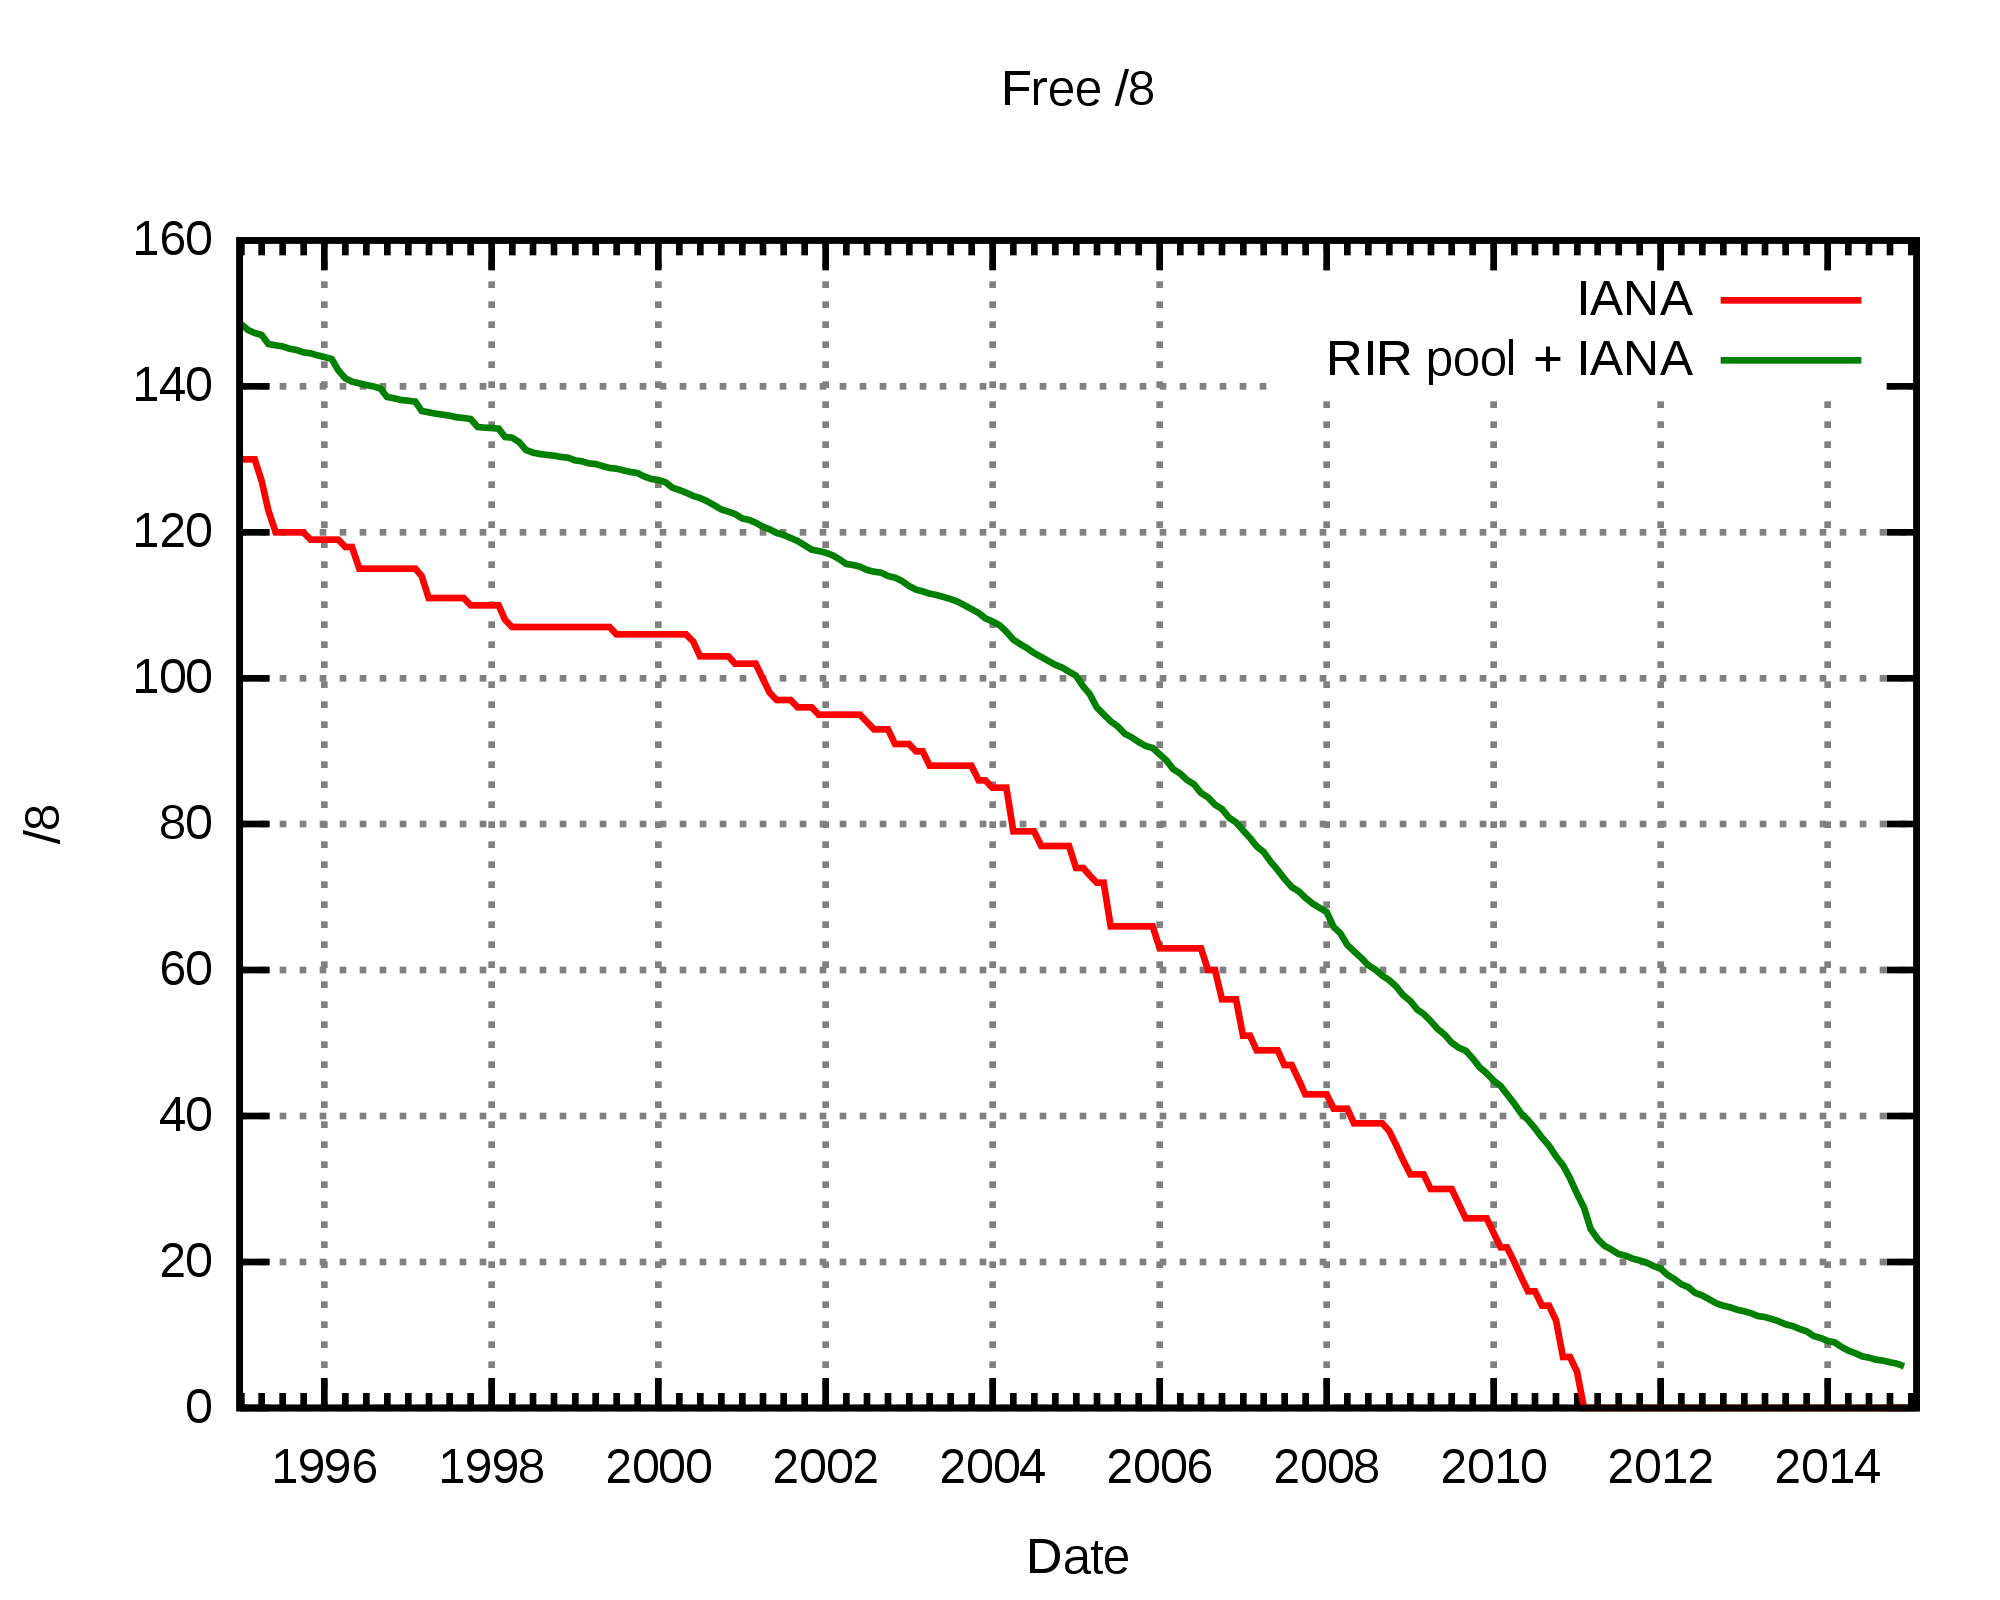
\includegraphics[width=\textwidth,keepaspectratio]{img/01}
	\source{https://upload.wikimedia.org/wikipedia/commons/c/cf/Ipv4-exhaust.svg}
	\caption{Wolne pule adresów IPv4 w czasie}
\end{figure}

Biorąc pod uwagę powyższe, na mocy Zasady Szufladkowej Dirichleta możemy
stwierdzić, że adres IPv4 nie jest już identyfikatorem, który mógłby unikatowo
identyfikować każde urządzenie podłączone do Internetu. W tym momencie warto
także zaznaczyć, że o ile nowy standard IPv6 pozwalałby na taką identyfikację,
to został on zaprojektowany z myślą o prywatności i posiada szereg rozszerzeń,
które w przyszłości (kiedy Internet w pełni przejdzie na adresację w wersji
szóstej) będą zapobiegać precyzyjnej identyfikacji.

\subsubsection{Cookies}
Małe porcje informacji zapisywane na urządzeniu użytkownika, w obszarze pamięci
trwałej przeglądarki, po interakcji ze stroną internetową, która je zapisuje.
Powstały głównie ze względu na potrzebę poprawienia doświadczeń użytkowników ze
stronami internetowymi, tak aby zapamiętywać pewien stan, o znaczeniu dla danej
sesji dla danego użytkownika (na przykład stan koszyka w sklepie internetowym).

Cookies dzielą się na tak zwane \emph{first-party cookies} i \emph{third-party
cookies}. O ile pierwsze z wymienionego podziału faktycznie desygnowane są do
tego aby spełniać wymienioną funkcję, to \emph{third-party cookies} mogą być
nadawane przez skrypty reklamowe (na przykład), umieszczone na serwującej je
stronie, dzięki czemu użytkownik może być śledzony w kontekście całej sieci
reklamowej. Ubogie mechanizmy kontroli cookies w przeglądarkach internetowych i
obawy związane z naruszaniem prywatności użytkowników przez śledzenie
wykorzystujące cookies, doprowadziły do powstania dyrektywy Unii Europejskiej
dotyczącej obowiązku informacyjnego, która zawiera m.in. obowiązek informowania
o polityce stosowania cookies. Doprowadziło to wcześniej także do powstania
rozszerzeń w przeglądarkach, takich jak nagłówek Do Not Track i Tryb Prywatny,
które w domyśle miały pomóc częściowo rozwiązać wspomniany problem.

Niektóre przeglądarki internetowe, takie jak Apple Safari (Intelligent Tracking
Prevention silnika WebKit) lub Mozilla Firefox wykorzystują obecnie natywne
mechanizmy inteligentnego blokowania \emph{third-party cookies}. Powstało także
wiele rozszerzeń do przeglądarek, które pozwalają blokować niechciane cookies.

\subsubsection{Inne techniki śledzenia użytkowników}
Fingerprinting urządzeń podłączonych do Internetu i przeglądarek internetowych,
to jedna ze zbioru wymyślnych technik, które zaczęto stosować ze względu na
ułomność i/lub postępujące ograniczenia technik wykorzystujących na przykład
adresy IP urządzeń i/lub cookies.

\section{Fingerprinting w branży komputerowej}
Fingerprinting to technika wykorzystywana w wielu obszarach w dyscyplinie
informatyki; fingerprinting urządzeń podłączonych do Internetu i przeglądarek
internetowych to tylko pewien wycinek zastosowań tej koncepcji. O ile podane na
początku tego rozdziału definicje ujmują fingerprint w sposób ogólny i także
taki, który pokrywa się z definicjami, które można znaleźć w publikacjach
dotyczących fingerprintingu urządzeń i przeglądarek, to definicje dotyczące
zastosowań fingerprintu innych bytów mogą być bardziej specyficzne czy też mogą
eksponować inne właściwości, charakterystyczne dla stosownych zastosowań.
Kolejne punkty służą jako referencja do ukazania jak szeroko wykorzystywana jest
omawiana koncepcja.

\subsection{Fingerprinting audio, wideo i algorytmy ACR}
Metody fingerprintingu akustycznego i cyfrowych materiałów wideo, znane także
jako algorytmy Automatic Content Recognition (ACR), powstały głównie ze względu
na potrzebę kontroli treści umieszczanych w serwisach internetowych pod kątem
potencjalnych naruszeń praw do wykorzystania. Algorytmy Automatic Content
Recognition są sparametryzowane w podobny sposób, co algorytmy fingerprintingu
urządzeń i przeglądarek, czyli istotny jest balans pomiędzy niepowtarzalnością a
stabilnością fingerprintu. Klasyfikacja fingerprintu audio lub wideo musi
działać w podobny sposób do zachowania ludzkiego moderatora, czyli w przypadku
kiedy materiał jest nieodróżnialny dla ludzkiego ucha lub oka jako ten, wobec
którego przeprowadzany jest proces rozpoznawania, to powinien on zostać
oflagowany. Proces wykorzystywany przez algorytmy ACR określany jest mianem
\emph{perceptual hashing}\footnote{Termin nie został przetłumaczony umyślnie, ze
	względu na fakt, iż polskie nazewnictwo jest w tym przypadku raczej
nieistniejące.}.

\subsection{Fingerprinting klucza publicznego}
